\documentclass[12pt]{article}
 
\newenvironment{sol}[1][Solution]{\begin{trivlist}\item[\hskip\labelsep {\bfseries #1:}]}{\end{trivlist}}
\usepackage{minted}
%\usemintedstyle{perldoc}
\usemintedstyle{vs}
\usepackage{graphicx}
\graphicspath{./}
\usepackage{diagbox}
\usepackage[margin=1in]{geometry} 
\usepackage{amsmath,amsthm,amssymb}
\usepackage{times,url}

\begin{document}
\renewcommand{\qedsymbol}{\filledbox}
\begin{center}
    \textbf{CS 5/7350} \\
    \textbf{Quiz \#2 Due Feb 22 for Completion Grade}
%replace X with the appropriate number
\end{center}
\begin{flushright}
\underline{Name \& ID: Bingying Liang \ 
48999397 \ \ \ \ \ \ \ \ \ \ \ \ \ \ \ CS5350? Yes / No $\surd$}
\end{flushright}

\begin{enumerate}
    \item \ [1.5 pts]Determine a Huffman encoding for each symbol in a message that contains:
    \underline{\ \ \ 11} 20 As, \\
    \underline{\ \ \ 10} 20 Bs, \\
    \underline{\ \ 011} 7 Ds, \\
    \underline{\ \ 010} 7 Es, \\
    \underline{0011} 3 Fs, \\
    \underline{0010} 3 Gs, \\
    \underline{0010} 2 Hs, \\
    \underline{0000} 2 Ks, \\
    
    How many bits are in the entire message if each symbol is encoded with 3 bits?
    \begin{sol}
    \begin{align*}
        (20+20+7+7+3+3+2+2) \times 3 = 64 \times 3 = 192 \ bits
    \end{align*}
    \end{sol}
    How many bits are in the entire Huffman coded message?
    \begin{sol}
    \hspace*{\fill}\\
        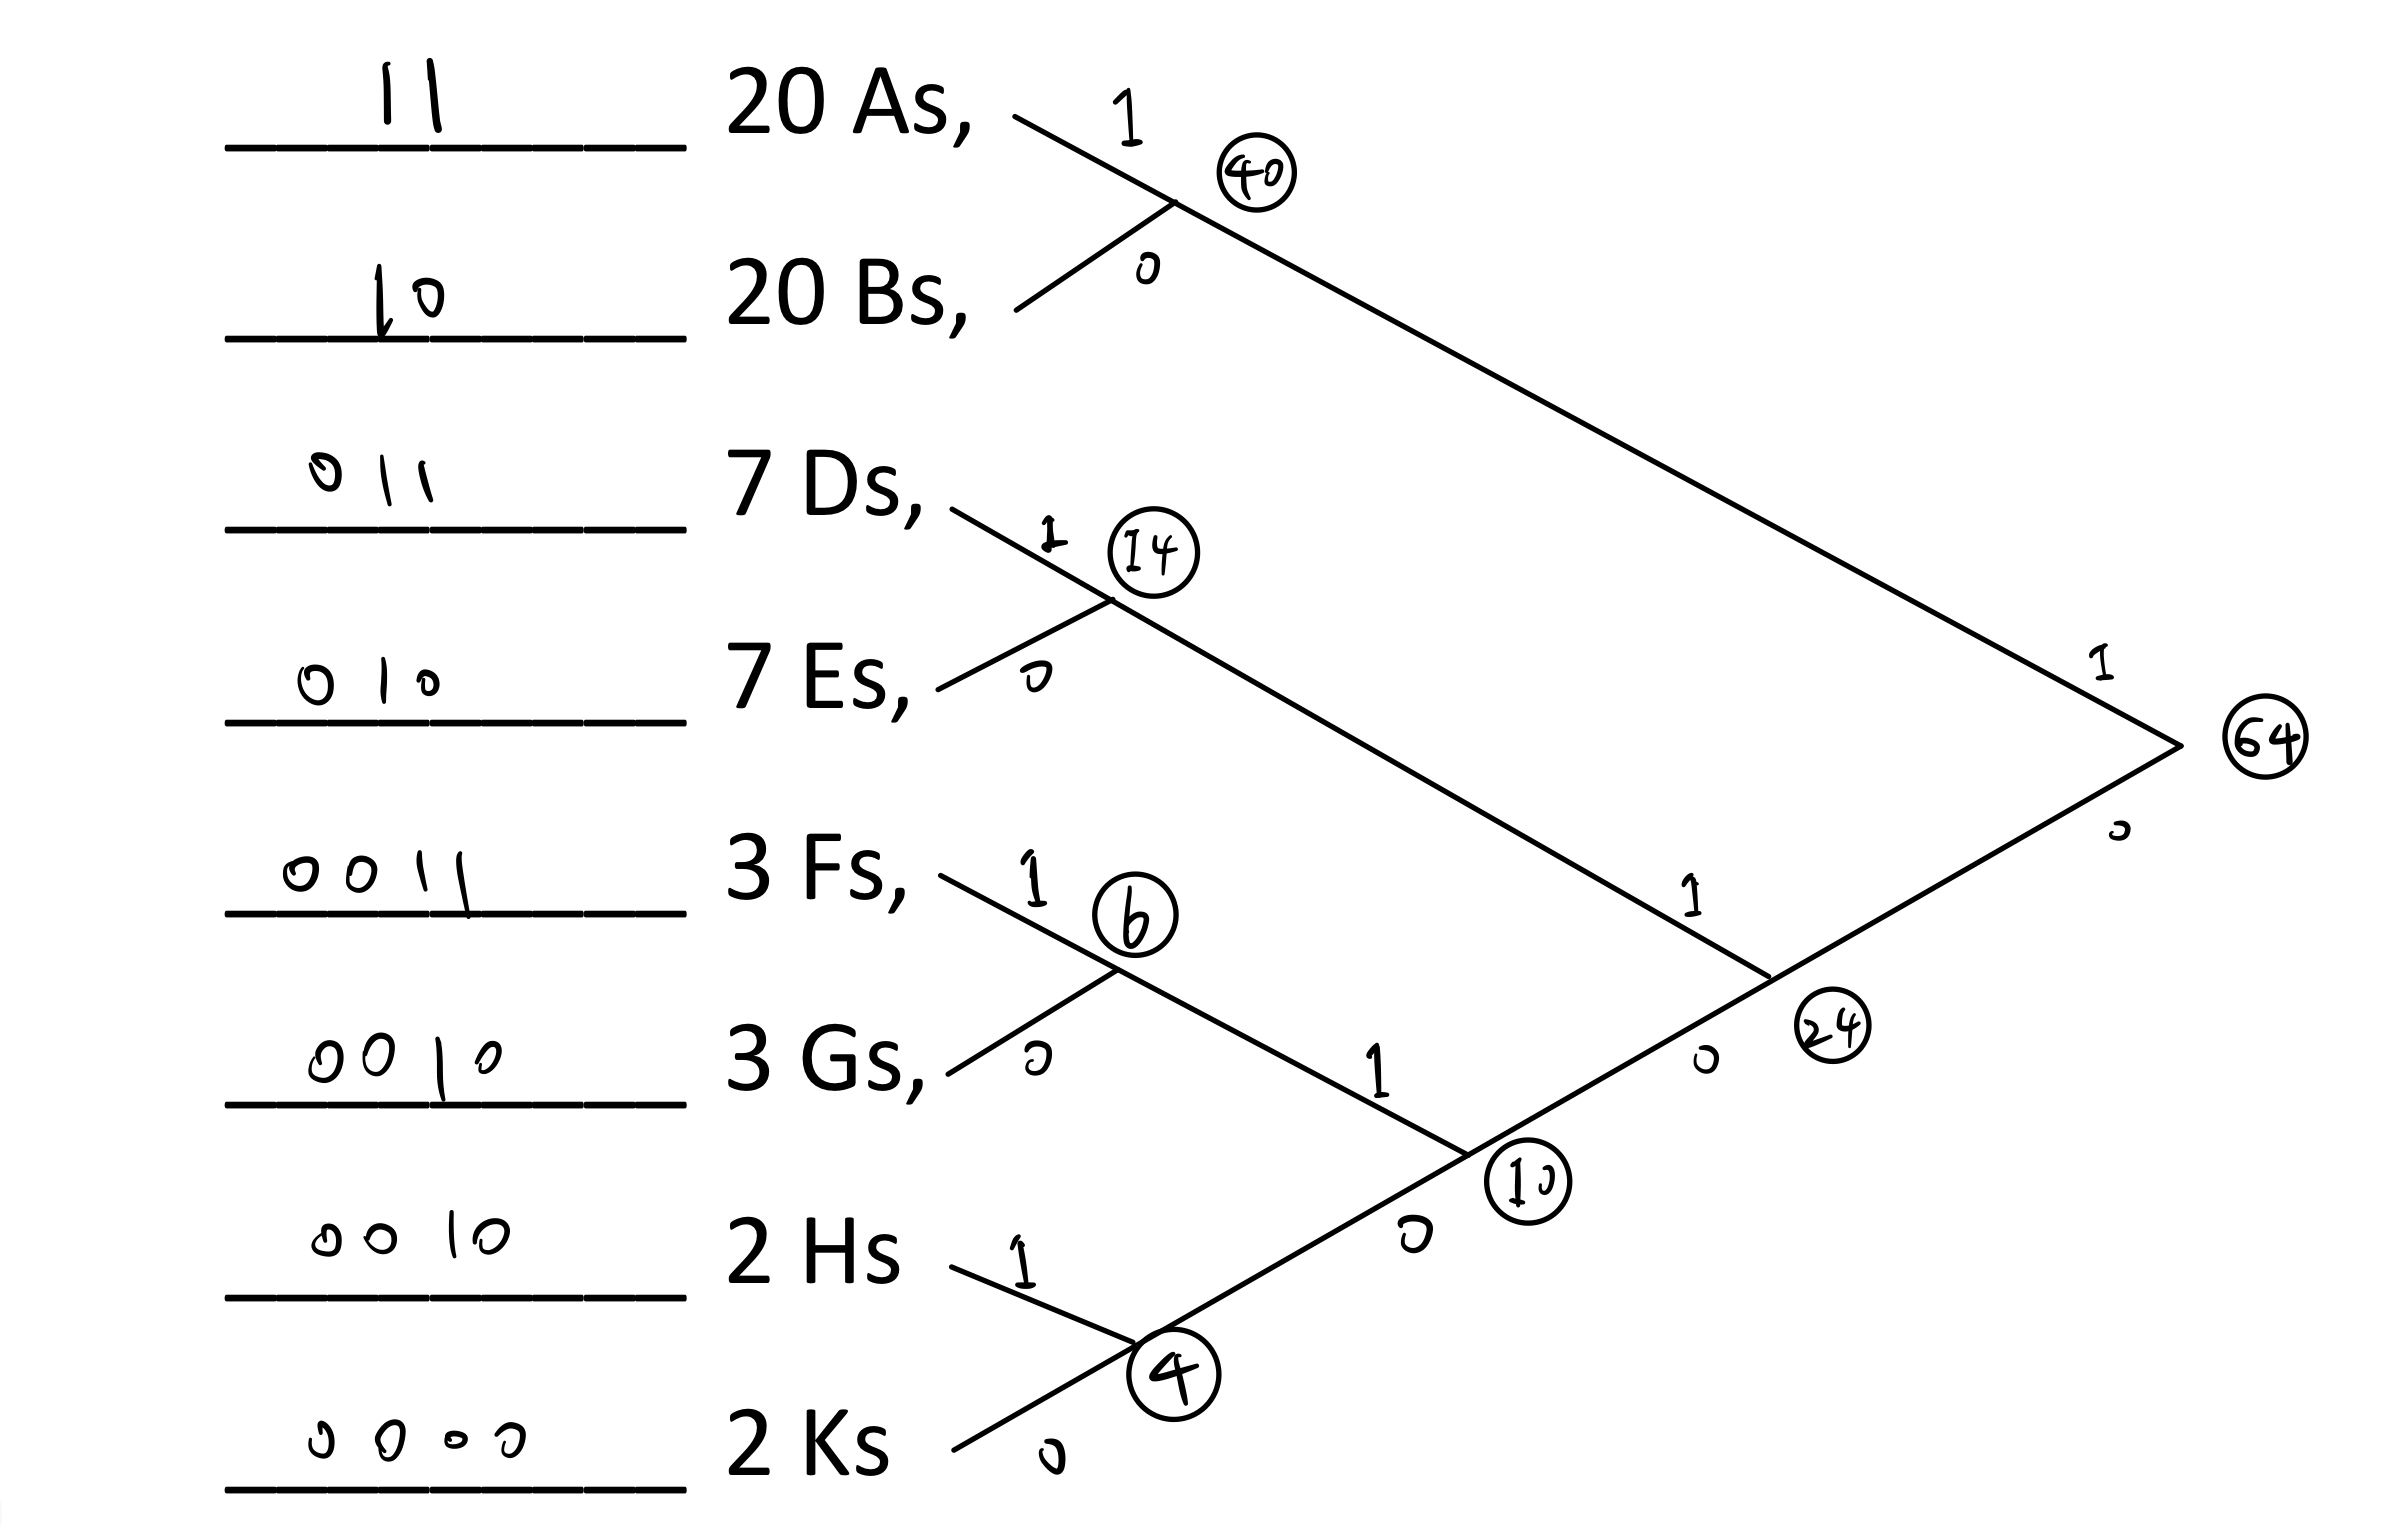
\includegraphics[width=0.5\textwidth]{p2.jpg}
        \begin{align*}
            (20+20) \times 2 + (7+7) \times 3 + (3+3+2+2)\times 4 = 80 + 42 + 40 = 162 \ bits  
        \end{align*}
    \end{sol}

    \item \ [2 pts] You run different programs for various value of "n" and create 4 tables of the runtimes. Given the Asymptoitc bounds that each of the tables support?\\
    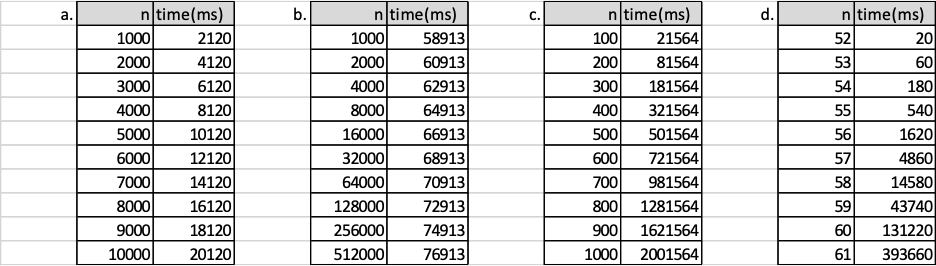
\includegraphics[width=0.9\textwidth]{p1.png}
    \begin{sol}
    \hspace*{\fill}\\
    \begin{enumerate}
        \item $\Theta(n)$. \\
        $\frac{10000}{1000} = 10, \frac{f(10000)}{f(1000)} = \frac{20120 \ ms}{2120 \ ms} = 9.49056603773585 \approx 9.5 \approx 10$ 
        \item $\Theta(log(n))$ \\
        $ \frac{f(512000)}{f(12800)} = \frac{76913 \ ms}{72913 \ ms} = 1.0548599015264768 \approx 1.1 \approx \frac{\log_2(512000)}{\log_2(128000)} =\frac{18.96578428}{16.96578428} = 1.1$\\
    
        \item $\Theta(n^2)$ \\
        $\frac{1000}{100} = 10, \frac{f(1000)}{f(100)}= \frac{2001564 \ ms}{21564 \ ms} = 92.81969949916528 \approx 9.59^2 \approx 10^2 $ \\
        $\frac{900}{300} = 3, \frac{f(900)}{f(300)} = \frac{1621564}{181564} = 8.931087660549448 \approx 9 = 3^2$
        \item $\Theta(3^n)$  \\ 
        $61-60=1 \frac{f(61)}{f(60)} = \frac{393660}{131220} = 3.0000685871056243 \approx 3^1$\\
        $60- 58 = 2 \frac{f(60)}{f(58)} = \frac{131220}{14580} = 9 = 3^2 $
    \end{enumerate}
    \end{sol}
    
    \item \ [1 pts] What is $(- \frac{1}{4}) \ modulo \ 7$?
    \begin{sol}
             \hspace*{\fill}\\
    \begin{align*}
        \begin{tabular}{|c|c|c|c|c|c|c|c|}
        \hline
        \diagbox{b}{$ab \bmod 7 $}{a} & 0 & 1 & 2 & 3 & 4 & \color{red}5 & 6 \\
        \hline
        0          & 0 & 0 & 0 & 0 & 0 & 0 & 0 \\
        \hline
        1          & 0 & 1 & 2 & 3 & 4 & 5 & 6 \\
        \hline
        2          & 0 & 2 & 4 & 6 & 1 & 3 & 5 \\
        \hline
        3          & 0 & 3 & 6 & 2 & 5 & 1 & 4 \\
        \hline
        \color{red}4  & 0 & 4 & 1 & 5 & 2 & \color{red}6 & 3 \\
        \hline
        5          & 0 & 5 & 3 & 1 & 6 & 1 & 2 \\
        \hline     
        6          & 0 & 6 & 5 & 4 & 3 & 2 & 1 \\
        \hline
        \end{tabular}
    \end{align*}

        \begin{align*}
            &\because (4 \times (-\frac{1}{4})) \% 7 = -1 \% 7 = 6, (4 \times 5) \% 7 = 6 \\
            &\therefore (-\frac{1}{4}) \% 7 = 5 
        \end{align*}
    \end{sol}

    \item \ [1 pts] Two people need to establish a secret key for encrypting communications. They agree to use a Diffie-Hellman key exchange with a modulus of 11 and decide on 2 as the base. Person A chooses a random value performs the appropriate computations and sends the value 6 to person B. Person B chooses a random value of 3 and performs the appropriate computations:
    \begin{enumerate}
        \item What is the value Person B sends to Person A
        \begin{sol}
            \begin{align*}
                B\rightarrow A: 2^3 \bmod \ 11 = 8 \bmod 11 = 8
            \end{align*}
        \end{sol}
        \item What is the shared secret key between Person A and Person B
        \begin{sol} 
            \begin{align*}
                (A \ sends \ to \ Person \ B) ^ 3 \bmod 11 = 6^3 \bmod 11 =  216 \bmod 11 = 7 
            \end{align*}
        \end{sol} 
    \end{enumerate}
    
\end{enumerate}

\end{document}
